\chapter{Lec 20-21-22 - Tree-Based Methods}

\section{Introduction}
In this chapter, we describe tree-based methods for regression and classification. These involve stratifying or segmenting the predictor space into a number of simple regions. In order to make a prediction for a given observation, we typically use the mean or the mode of the training observations in the region to which it belongs.\\\\
Tree-based methods are simple and useful for interpretation. However,
they typically are not competitive with the best supervised learning approaches in terms of prediction accuracy. Hence in this chapter we also introduce \textit{bagging} and \textit{random forests}. Each of these approaches involves producing multiple trees which are then combined to yield a single consensus prediction.

\section{The Basics of Decision Trees}
Decision trees can be applied to both regression and classification problems.
We first consider regression problems, and then move on to classification.

\subsection{Regression Trees}
In order to motivate regression trees, we begin with a simple example.

\subsubsection{Predicting Baseball Players’ Salaries Using Regression Trees}
We use the Hitters data set to predict a baseball player’s \textit{Salary} based on \textit{Years} (the number of years that he has played in the major leagues) and \textit{Hits} (the number of hits that he made in the previous year). We first remove observations that are missing \textit{Salary} values, and log-transform \textit{Salary} so that its distribution has more of a typical bell-shape. The Figure below  shows a regression tree fit to this data. It consists of a series of splitting rules, starting at the top of the tree. The top split assigns observations having $Years<4.5$ to the left branch.
\begin{center}
    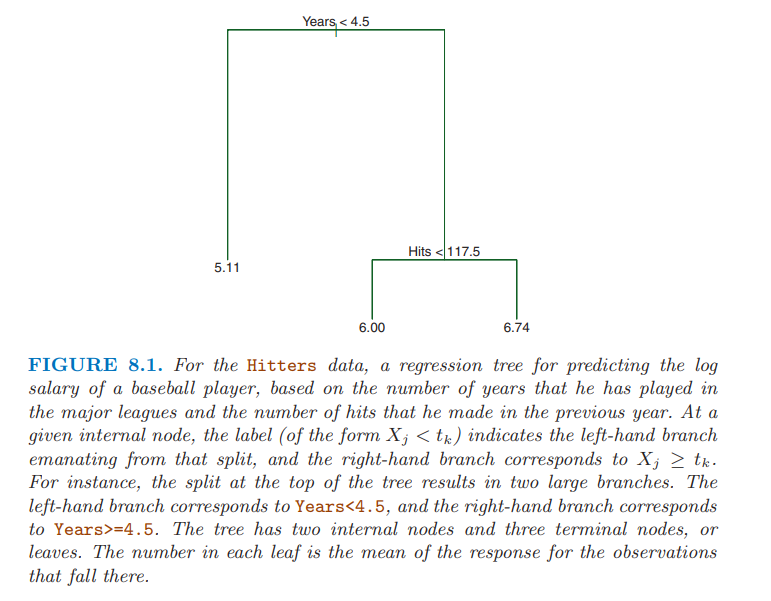
\includegraphics[scale=0.7]{images/reg-tree.png}
\end{center}
The predicted salary for these players is given by the mean response value for the players in the data set with $Years<4.5$. Overall, the tree stratifies
or segments the players into three regions of predictor space: players who have played for four or fewer years, players who have played for five or more years and who made fewer than 118 hits last year, and players who have played for five or more years and who made at least 118 hits last year. The figure below  illustrates the regions as a function of \textit{Years} and \textit{Hits}
\begin{center}
    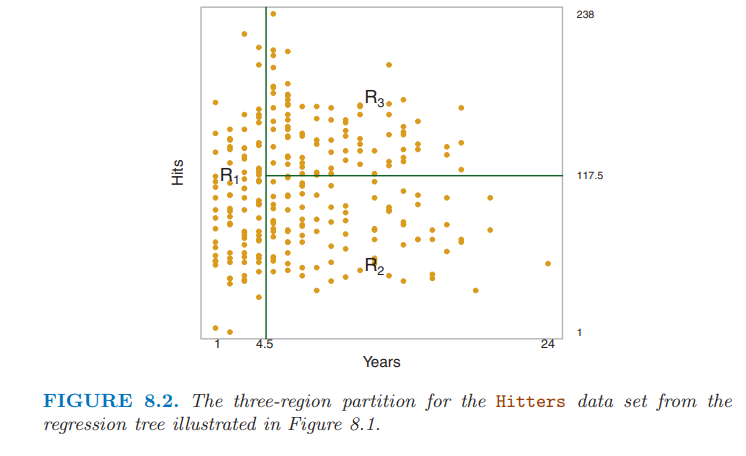
\includegraphics[scale=0.7]{images/reg-tree-2.png}
\end{center}
We might interpret this regression tree as follows: \textit{Years} is the most important factor in determining \textit{Salary}, and players with less experience earn lower salaries than more experienced players. Given that a player is less experienced, the number of hits that he made in the previous year seems to play little role in his salary. But among players who have been in the major leagues for five or more years, the number of hits made in the previous year does affect salary, and players who made more hits last year tend to have higher salaries.

\subsubsection{Prediction via Stratification of the Feature Space}
We now discuss the process of building a regression tree. Roughly speaking,
there are two steps.
\begin{enumerate}
    \item  We divide the predictor space, that is, the set of possible values for $X_1, X_2,...,X_p$, into $J$ distinct and non-overlapping regions, $R_1, R_2,...,R_J$.

    \item For every observation that falls into the region $R_j$ , we make the same prediction, which is simply the mean of the response values for the training observations in $R_j$.
\end{enumerate}
How do we construct the regions $R_1,...,R_J$? In theory, the regions could have any shape. However, we choose to divide the predictor space into high-dimensional rectangles, or boxes, for simplicity and for ease of interpretation of the resulting predictive model. The goal is to find boxes $R_1,...,R_J$ that minimize the RSS, given by
\begin{equation}
    \sum_{j=1}^J\sum_{i \in R_j}(y_i - \hat{y}_{R_j})^2
\end{equation}
where $\hat{y}_{R_j}$ is the mean response for the training observations within the $j$th box. Unfortunately, it is computationally infeasible to consider every
possible partition of the feature space into $J$ boxes. For this reason, we take
a \textit{top-down}, \textit{greedy} approach that is known as \textit{recursive binary splitting}. The approach is top-down because it begins at the top of the tree  and then successively splits the predictor space; each split is indicated via two new branches further down on the tree. It is greedy because at each step of the tree-building process, the best split is made at that particular step, rather than looking ahead and picking a split that will lead to a better tree in some future step.\\\\
In order to perform recursive binary splitting, we first select the predictor $X_j$ and the cutpoint $s$ such that splitting the predictor space into the regions $\{X|X_j < s\}$ and $\{X|X_j \geq s\}$ leads to the greatest possible
reduction in RSS. In greater detail, for any $j$ and $s$, we define the pair of half-planes
\[R_1(j,s) = \{X|X_j < s\} \quad \text{and} \quad R_2(j, s) = \{X|X_j \geq s\}\]
and we seek the value of j and s that minimize the equation
\begin{equation}
    \sum_{i:x_i \in R_1(j, s)}(y_i - \hat{y}_{R_1})^2 + \sum_{i:x_i \in R_2(j, s)}(y_i - \hat{y}_{R_2})^2
    \label{rec-split}
\end{equation}
Finding the values of j and s that minimize \ref{rec-split} can be done quite quickly, especially when the number of features $p$ is not too large. Next, we repeat the process, looking for the best predictor and best cutpoint in order to split the data further so as to minimize the RSS within each of the resulting regions. However, this time, instead of splitting the entire predictor space, we split one of the two previously identified regions. We now have three regions. Again, we look to split one of these three regions further, so as to minimize the RSS. The process continues until a stopping criterion is reached; for instance, we may continue until no region contains more than five observations.

\subsubsection{Tree Pruning}
The process described above may produce good predictions on the training set, but is likely to overfit the data. This is because the resulting tree might be too complex. A smaller tree with fewer splits might lead to lower variance and better interpretation at the cost of a little bias. One possible alternative to the process described above is to build the tree only so long as the decrease in the RSS due to each split exceeds some (high) threshold. This strategy will result in smaller trees, but is too short-sighted since a seemingly worthless split early on in the tree might be followed by a very good split. Therefore, a better strategy is to grow a very large tree $T_0$, and then \textit{prune} it back in order to obtain a subtree. Intuitively, our goal is to select a subtree that leads to the lowest test error rate. Given a subtree, we can estimate its test error using cross-validation or the validation set approach. However, estimating the cross-validation error for every possible subtree would be too cumbersome, since there is an extremely large number of possible subtrees. Instead, we need a way to select a small set of subtrees for consideration.\\\\
\textit{Cost complexity pruning} gives us a way to do just this. Rather than considering every possible subtree, we consider a sequence of trees indexed by a nonnegative tuning parameter $\alpha$. For each value of $\alpha$ there corresponds a subtree $T \subset T_0$ such that
\begin{equation}
    \sum_{m=1}^{|T|}\sum_{i:x_i \in R_m}(y_i - \hat{y}_{R_m})^2 + \alpha|T|
    \label{pruning}
\end{equation}
is minimized. Here $|T|$ indicates the number of terminal nodes of the tree $T$. The tuning parameter $\alpha$ controls a trade-off between the subtree’s complexity and its fit to the training data. Equation \ref{pruning} is reminiscent of the lasso, in which a similar formulation was used in order to control the complexity of a linear model.\\\\
It turns out that as we increase $\alpha$ from zero in \ref{pruning}, branches get pruned from the tree in a nested and predictable fashion, so obtaining the whole sequence of subtrees as a function of $\alpha$ is easy. We can select a value of $\alpha$ using a validation set or using cross-validation. This process is summarized in the Algorithm below.
\begin{center}
    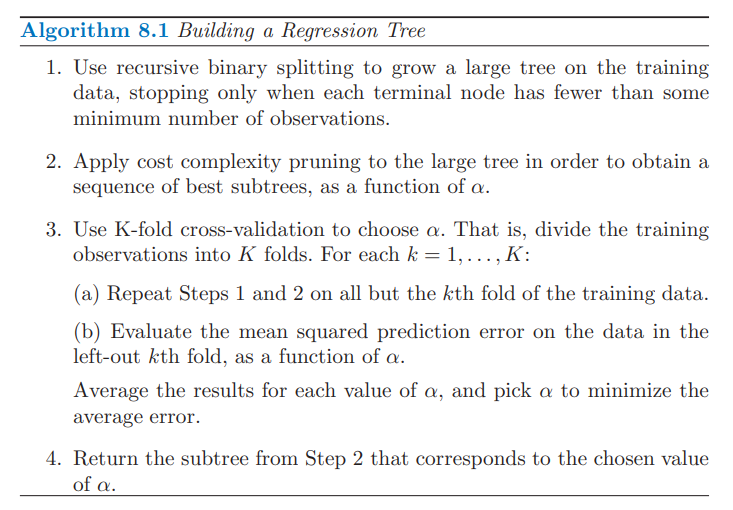
\includegraphics[scale=0.7]{images/pruning.png}
\end{center}

\subsection{Classification Trees}
A \textit{classification tree} is very similar to a regression tree, except that it is used to predict a qualitative response rather than a quantitative one. Recall that  for a regression tree, the predicted response for an observation is given by the mean response of the training observations that belong to the same terminal node. In contrast, for a classification tree, we predict that each observation belongs to the most commonly occurring class of training observations in the region to which it belongs.\\\\
In the classification setting, RSS cannot be used as a criterion for making the binary splits. A natural alternative to RSS is the \textit{classification error rate}, which is simply the fraction of the training observations in that region that do not belong to the most common class:
\begin{equation}
    E = 1 - max_k(\hat{p}_{mk})
\end{equation}
Here $\hat{p}_{mk}$ represents the proportion of training observations in the $m$th region that are from the $k$th class. However, it turns out that classification error is not sufficiently sensitive for tree-growing, and in practice two other measures are preferable.
\\\\
The \textit{Gini index} is defined by
\begin{equation}
    G = \sum_{k=1}^K \hat{p}_{mk}(1 - \hat{p}_{mk})
\end{equation}
a measure of total variance across the $K$ classes. It is not hard to see
that the Gini index takes on a small value if all of the $\hat{p}_{mk}$’s are close to zero or one. For this reason the Gini index is referred to as a measure of \textit{node purity}, a small value indicates that a node contains predominantly observations from a single class.\\\\
An alternative to the Gini index is cross-entropy, given by
\begin{equation}
    D = -\sum_{k=1}^K \hat{p}_{mk} log\, (\hat{p}_{mk})
\end{equation}
One can show that the cross-entropy will take on a value near zero if the $\hat{p}_{mk}$’s are all near zero or near one. Therefore, like the Gini index, the cross-entropy will take on a small value if the $m$th node is pure.\\\\
When building a classification tree, either the Gini index or the cross-entropy are typically used to evaluate the quality of a particular split. Any of these three approaches might be used when pruning the tree, but the classification error rate is preferable if prediction accuracy of the final pruned tree is the goal.\\\\
In our discussion thus far, we have assumed that the predictor variables take on continuous values. However, decision trees can be constructed even in the presence of qualitative predictor variables.\\\\
The figure below has a surprising characteristic: some of the splits yield two terminal nodes that have the same predicted value.
\begin{center}
    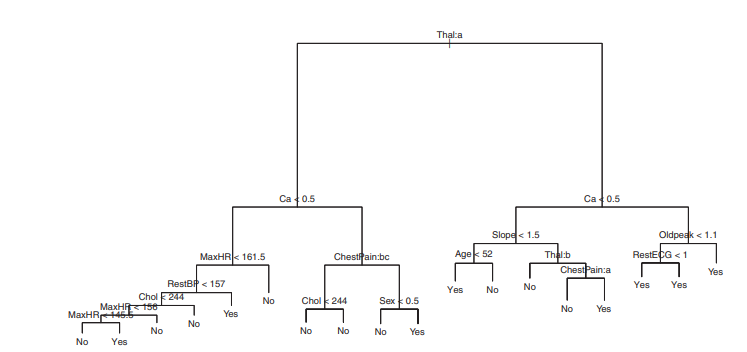
\includegraphics[scale=0.8]{images/classification-tree.png}
\end{center}
For instance, consider the split $RestECG<1$ near the bottom right of the unpruned tree. Regardless of the value of \textit{RestECG}, a response value of \textit{Yes} is predicted for those observations. Why, then, is the split performed at all? The split is performed because it leads to increased \textit{node purity}. That is, all 9 of the observations corresponding to the right-hand leaf have a response value of \textit{Yes}, whereas 7/11 of those corresponding to the left-hand leaf have a response value of \textit{Yes}. Why is node purity important? Suppose that we have a test observation that belongs to the region given by that right-hand leaf. Then we can be pretty certain that its response value is \textit{Yes}. In contrast, if a test observation belongs to the region given by the left-hand leaf, then its response value is probably \textit{Yes}, but we are much less certain. Even though the split \textit{RestECG<1} does not reduce the classification error, it improves the Gini index and the cross-entropy, which are more sensitive to node purity.

\subsection{Trees Versus Linear Models}
Regression and classification trees have a very different flavor from the more
classical approaches for regression and classification presented in the previous Chapters, such as linear regression. Which model is better? It depends on the problem at hand. If the relationship between the features and the response is well approximated by a linear model, then an approach such as linear regression
will likely work well, and will outperform a method such as a regression tree that does not exploit this linear structure. If instead there is a highly
non-linear and complex relationship between the features and the response, then decision trees may outperform classical approaches. Furthermore, in certain settings, prediction using a tree may be preferred for the sake of interpretability and visualization.
\begin{center}
    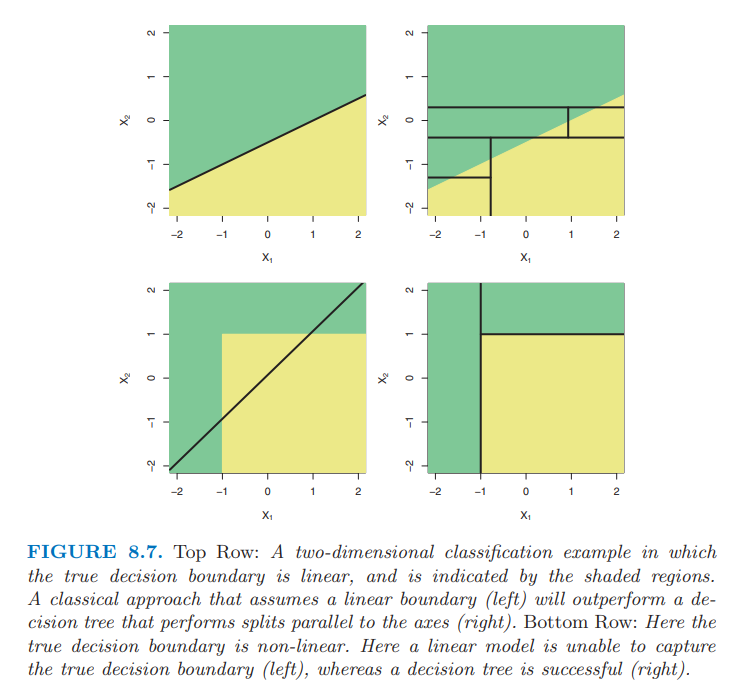
\includegraphics[scale=.7]{images/lin-reg-vs-reg-tree.png}
\end{center}

\subsection{Advantages and Disadvantages of Trees}
Decision trees for regression and classification have a number of advantages
over the more classical approaches:\\\\
\textbf{Pros:}
\begin{itemize}
    \item Trees are very easy to explain to people.
    
    \item Some people believe that decision trees more closely mirror human decision-making than do the regression and classification approaches.

    \item Trees can be displayed graphically.

    \item Trees can easily handle qualitative predictors without the need to create dummy variables. 
\end{itemize}
\textbf{Cons:}
\begin{itemize}
    \item Unfortunately, trees generally do not have the same level of predictive accuracy as some of the other regression and classification approaches.
\end{itemize}
However, by aggregating many decision trees, using methods like \textit{bagging} and \textit{random forests}, the predictive performance of trees can be
substantially improved.

\section{Bagging and Random Forests}
\subsection{Bagging}
The decision trees discussed previously suffer from high variance. This means that if we split the training data into two parts at random, and fit a decision tree to both halves, the results that we get could be quite different. In contrast, a procedure with low variance will yield similar results if applied repeatedly to distinct data sets. \textit{Bootstrap aggregation}, or \textit{bagging}, is a general-purpose procedure for reducing the variance of a statistical learning method; we introduce it here because it is particularly useful and frequently used in the context of decision trees.\\\\
Recall that given a set of $n$ independent observations $Z_1,...,Z_n$, each
with variance $\sigma^2$, the variance of the mean $\Bar{Z}$ of the observations is given by $\sigma^2/n$. In other words, averaging a set of observations reduces variance. Hence a natural way to reduce the variance and hence increase the prediction accuracy of a statistical learning method is to take many training sets from the population, build a separate prediction model using each training set, and average the resulting predictions. Of course, this is not practical because we generally do not have access to multiple training sets. Instead, we can \textit{bootstrap}, by taking repeated samples from the (single) training data set. In this approach we generate $B$ different bootstrapped training data sets. We then train our method on the $b$th bootstrapped training set, and finally average all the predictions. 
\\\\
While bagging can improve predictions for many regression methods, it is particularly useful for decision trees. Each of the $B$ trees is grown deep (on the $b$th bootstrapped training set), and are not pruned. Hence each individual tree has high variance, but low bias. Averaging these $B$ trees reduces the variance. How can bagging be extended to a classification problem where $Y$ is qualitative? In that situation, there are a few possible approaches, but the simplest is as follows. For a given test observation, we can record the class predicted by each of the B trees, and take a \textit{majority vote}: the overall prediction is the most commonly occurring class among the $B$ predictions.

\subsubsection{Out-of-Bag Error Estimation}
It turns out that there is a very straightforward way to estimate the test error of a bagged model, without the need to perform cross-validation or the validation set approach. One can show that on average, each bagged tree makes use of around two-thirds of the observations. The remaining one-third of the observations not used to fit a given bagged tree are referred to as the out-of-bag (OOB) observations. We can predict the response for the $i$th observation using each of the trees in which that observation was OOB. This will yield around $B/3$ predictions for the $i$th observation. In order to obtain a single prediction for the $i$th observation, we can average these predicted responses (or can take a majority vote). This leads to a single OOB prediction for the $i$th observation. An OOB prediction can be obtained in this way for each of the $n$ observations, from which the overall OOB MSE or classification error can be computed. The resulting OOB error is a valid estimate of the test error for the bagged model, since the response for each observation is predicted using only the trees that were not fit using that observation.

\subsubsection{Variable Importance Measures}
As we have discussed, bagging typically results in improved accuracy over
prediction using a single tree. Unfortunately, however, it can be difficult to
interpret the resulting model. When we bag a large number of trees, it is no longer possible to represent the resulting statistical learning procedure using a single tree. Thus, bagging improves prediction accuracy at the expense of interpretability.\\\\
Although the collection of bagged trees is much more difficult to interpret
than a single tree, one can obtain an overall summary of the importance of
each predictor using the RSS (or the Gini index). In the case of bagging regression trees, we can record the total amount that the RSS  is decreased due to splits over a given predictor, averaged over all $B$ trees. A large value indicates an important predictor.

\subsection{Random Forests}
Random forests provide an improvement over bagged trees by way of a small tweak that \textit{decorrelates} the trees. As in bagging, we build a number of decision trees on bootstrapped training samples. But when building these decision trees, each time a split in a tree is considered, a random sample of $m$ predictors is chosen as split candidates from the full set of $p$ predictors. The split is allowed to use only one of those $m$ predictors. Typically we choose $m \approx \sqrt{p}$.\\\\
In other words, in building a random forest, at each split in the tree,
the algorithm is not even allowed to consider a majority of the available
predictors. This may sound crazy, but it has a clever rationale. Suppose that there is one very strong predictor in the data set, along with a number of other moderately strong predictors. Then in the collection of bagged trees, most or all of the trees will use this strong predictor in the top split. Consequently, all of the bagged trees will look quite similar to each other. Hence the predictions from the bagged trees will be highly correlated. Unfortunately,  averaging many highly correlated quantities does not lead to as large of a reduction in variance as averaging many uncorrelated quantities.\\\\
Random forests overcome this problem by forcing each split to consider only a subset of the predictors. Therefore, on average $(p - m)/p$ of the splits will not even consider the strong predictor, and so other predictors will have more of a chance. Using a small value of $m$ in building a random forest will typically be helpful when we have a large number of correlated predictors.
